\documentclass[thesis.tex]{subfiles}
\begin{document}
\chapter{Background}

\section{SecPAL}

SecPAL is an authorization language developed by Becker~\etal~to
describe policies and delegation chains surrounding distributed
services~\cite{becker_secpal:_2006}. It was designed as a high-level
human-readable language that allowed the policy specification and
maintenance to be separated from the implementation mechanisms.

SecPAL was designed to improve over previous high-level languages in
several areas.  It was designed to be more expressive than
XrML~\cite{kolovski_logic-based_2007},
SPKI/SDSI~\cite{ellison_spki_1999}, and Delegation
Logic~\cite{li_delegation_2003}; and more readable than
XACML~\cite{oasis_extensible_2013} and other XML-based policy
languages.  Furthermore it was designed to be intuitive and
unambiguous with precise semantics unlike other languages (most notably
XACML) which had natural language descriptions with ambiguous and
inconsistent specifications that had been retrofitted to the language
instead of being designed with the language in the first
place~\cite{bryans_reasoning_2005,ramli_logic_2014,masi_formalisation_2012}.

SecPAL's original application was to model and enforce access control
policies in grid computing systems~\cite{becker_secpal:_2006}.  In
this dissertation we describe how the language can be extended to
describe the policies surrounding the mobile ecosystem.

At its core, SecPAL is a language with a simple grammar
(\autoref{fig:secpal-grammar}) and three evaluation rules
(\autoref{fig:secpal-rules}). The language's simplicity makes it easy
to apply to a new domain by instantiating it with predicates and
constraints that describe the domain. This simplicity does not come at
the cost of its expressiveness. SecPAL supports delegation (by using
\emph{can-say} verbs), role and attribute based policies (by using
\emph{can-act-as} verbs) and arbitrary constraints.

\begin{figure}
  \newcommand{\bracetext}[1]{\text{\sffamily #1}}
  \newcommand{\smalltext}[1]{\text{\ttfamily\small #1}}
  \centering
  \begin{equation*}
    \begin{array}{r l}
      \overbrace{\smalltext{`user'}}^{\bracetext{speaker}} &
                                                             \smalltext{ says }\overbrace{\overbrace{\smalltext{ App }}^{\bracetext{subject}}\overbrace{\smalltext{ isRunnable}}^{\bracetext{predicate}}}^{\bracetext{fact}} \\
                                                           & \overbrace{\smalltext{ if App isFree}}^{\bracetext{condition}} \\
                                                           & \overbrace{\smalltext{ where hasPermission(App, `INTERNET') = true}}^{\bracetext{constraint}}.
    \end{array}
  \end{equation*}
  \caption{Structure of a SecPAL assertion.}
  \label{fig:assertion}
\end{figure}

\newcommand{\bnfcomment}[1]{\slshape{\sffamily(#1)}}
\newcommand{\secpal}[1]{\texttt{#1}}
\begin{figure}\footnotesize\centering
  \begin{tabular}{r r l c}
    AC         & $\Coloneqq$ & assertion$_1$ \dots assertion$_n$                      & \bnfcomment{assertion context} \\
    assertion  & $\Coloneqq$ & e \secpal{says} claim.                          \\
    e          & $\Coloneqq$ & \secpal{x}                                       & \bnfcomment{variables}         \\
               & $\vert$     & \secpal{A}                                       & \bnfcomment{constants}         \\
    predicate  & $\Coloneqq$ & \secpal{has} $\vert$ \secpal{can} $\vert$ \dots  & \bnfcomment{predicates}        \\
    D          & $\Coloneqq$ & 0                                                & \bnfcomment{no delegation}     \\
               & $\vert$     & $\infty$                                         & \bnfcomment{unbounded delegation}        \\
    vp         & $\Coloneqq$ & predicate e$_1$ \dots e$_n$                           & \bnfcomment{verb phrase}       \\
               & $\vert$     & \secpal{can-say}$_D$ fact                       \\
               & $\vert$     & \secpal{can-act-as}  e                          \\
    f          & $\Coloneqq$ & e vp                                             & \bnfcomment{fact}              \\
    claim      & $\Coloneqq$ & f \secpal{if} f$_1$,\dots, f$_n$; c             \\
    c          & $\Coloneqq$ & $\top$                                           & \bnfcomment{no constraint}     \\
               & $\vert$     & e$^\prime_1 =$ e$^\prime_2$                      & \bnfcomment{constraints}       \\
               & $\vert$     & \dots                                           \\
    e$^\prime$ & $\Coloneqq$ & e $\vert$ function(e$_1$,\dots e$_n$)           \\
  \end{tabular}
  \caption{BNF description of SecPAL.}
  \label{fig:secpal-grammar}
\end{figure}


\begin{figure}
  \centering
  \begin{eqnarray*}
    \infer[\textsf{\scriptsize cond}]{%
      AC, D \models A\textsf{~says~}fact\theta
    }{%
      \begin{array}[c]{c}
        \left(A\textsf{~says~}\textit{fact}\textsf{~if~}\textit{fact}_1, \ldots, \textit{fact}_k, c\right) \in AC \\
        AC,D\models A\textsf{~says~}\textit{fact}_i\theta \; \forall i \in \{1\cdots k\}
      \end{array}
      & \models{c\theta}
      & \textsf{vars}(\textit{fact}\theta) = \emptyset)
    }\\
    \infer[\textsf{\scriptsize can say}]{%
      AC, \infty \models A\textsf{~says~}\textit{fact}
    }{%
      AC, \infty \models A\textsf{~says~}B\textsf{~can~say}_D \textit{fact}
      & AC, D \models B\textsf{~says~}\textit{fact}
    } \\
    \infer[\textsf{\scriptsize can act as}]{%
      AC, D \models A\textsf{~says~}B~\textit{verbphrase}
    }{%
      AC, D \models A\textsf{~says~}B\textsf{~can~act~as~}C
      & AC, D \models A\textsf{~says~}C~\textit{verbphrase}
    }
  \end{eqnarray*}
  \caption[Inference rules used to evaluate {SecPAL}.]{The inference rules used to evaluate {SecPAL}. All {SecPAL} rules are
  evaluated in the context of a set of other assertions $AC$ as well as an
  allowed level of delegation $D$ which may be $0$ or $\infty$.}
\label{fig:secpal-rules}
\end{figure}

\begin{figure}\centering\sffamily\footnotesize
  \begin{tabular}{c l p{0.6\linewidth}}
    \toprule
    \multirow{3}{*}{\rotatebox{90}{Concepts\hspace{1em}}} & $AC,\theta \vdash q$                     & Defining relation. A query assertion $q$ is valid given the assertions contained in the assertion context $AC$ and a variable substitution $\theta$. \\
    &$\epsilon$                               & The empty substitution. \\
    
    \midrule
    \multirow{5}{*}{\rotatebox{90}{Definitions}} &
    1. $AC,\theta \vdash \overbrace{e \text{ says } fact}^q.$  & if $AC,\infty \models e\theta \text{ says } fact\theta$ and $dom(\theta) \subseteq vars(e \text{ says } fact)$                                       \\
    &2. $AC,\theta_1\theta_2 \vdash q_1, q_2$    & if $AC,\theta_1 \vdash q_1$ and $AC,\theta_2 \vdash_2 q_2\theta_1$                                                                                   \\
    &3. $AC,\theta \vdash q_1 \text{ or } q_2$   & if $AC,\theta \vdash q_1$ or $AC,\theta \vdash q_2$                                                                                                  \\
    &4. $AC,\epsilon \vdash \mathsf{not}(q)$     & if $AC,\epsilon \not\vdash q$ and $vars(q) = \emptyset$                                                                                              \\
    &5. $AC,\epsilon \vdash c$                   & if $\models c$                                                                                                                                       \\
    \bottomrule                             \\
  \end{tabular}
  \caption[SecPAL's semantics.]{SecPAL's semantics as described by Becker~\cite{becker_secpal:_2006}.}
  \label{fig:secpal-semantics}
\end{figure}

SecPAL's semantics are given in \autoref{fig:secpal-semantics}.  A
query $q$ to a SecPAL program (which is a collection of facts and
relationships called the \emph{assertion context} or \emph{AC}) asks
if there exists a renaming $\theta$ such that the rules of SecPAL can
be used to derive the, possibly renamed, query ($AC,\theta \vdash q$
if $AC,\infty \models q\theta$)\footnote{$\vdash$ describes if a query
  is valid with respect to an AC, whereas $\models$ says there is a
  valid proof for a SecPAL using the rules of SecPAL.  Conjugation,
  disjunction and negation are allowed within a query, but not when
  evaluating SecPAL.}.  The renaming must be specific and talk only of
the variables contained in the query, conjunction and disjunction work
as expected.  Negation is only allowed in an extremely limited form: a
query can be not true if it contains no variables and there is no way
to show that the AC supports the query.  This limited form means that
queries remain decidable: the rules inside the AC are not permitted to
use negation.

SecPAL was later extended to add universal quantification, and the
possibility of dynamic assertion retrieval (they defined a safety
condition, but didn't describe a protocol for retrieving assertions).
They also abandoned the roles to use exclusively depth bounded
delegation (citing a lack of uses in
practice)~\cite{moritz_y_becker_secpal:_2009}.  These ideas would be
expanded to create a new language called
DKAL~\cite{gurevich_dkal:_2008}.  Gruevich~\etal~showed how SecPAL
policies could be translated into DKAL
policies~\cite{gurevich_dkal:_2008} so any SecPAL-based policies could
be updated to DKAL.  We don't use these additional features in this
thesis as we did not need the additional expressiveness they provide
to adequately describe the policies in the mobile ecosystem.

\subsection{Delegation in SecPAL}

A key feature of SecPAL is the ability to delegate statements. SecPAL was
designed to make access control decisions over large networks. Rather than have
a centralized decision server where all decisions are made, SecPAL allows
information to be shared through assertions signed by their speaker. This allows
different principals to be responsible for different decisions and make
decisions independently. An example of this, expanded from one given by
Becker~\cite{becker_secpal:_2006}, is of a researcher attempting to run a query
on a cluster, using data from a fileserver (\autoref{fig:delegation-example}).

\begin{figure}
  \centering
  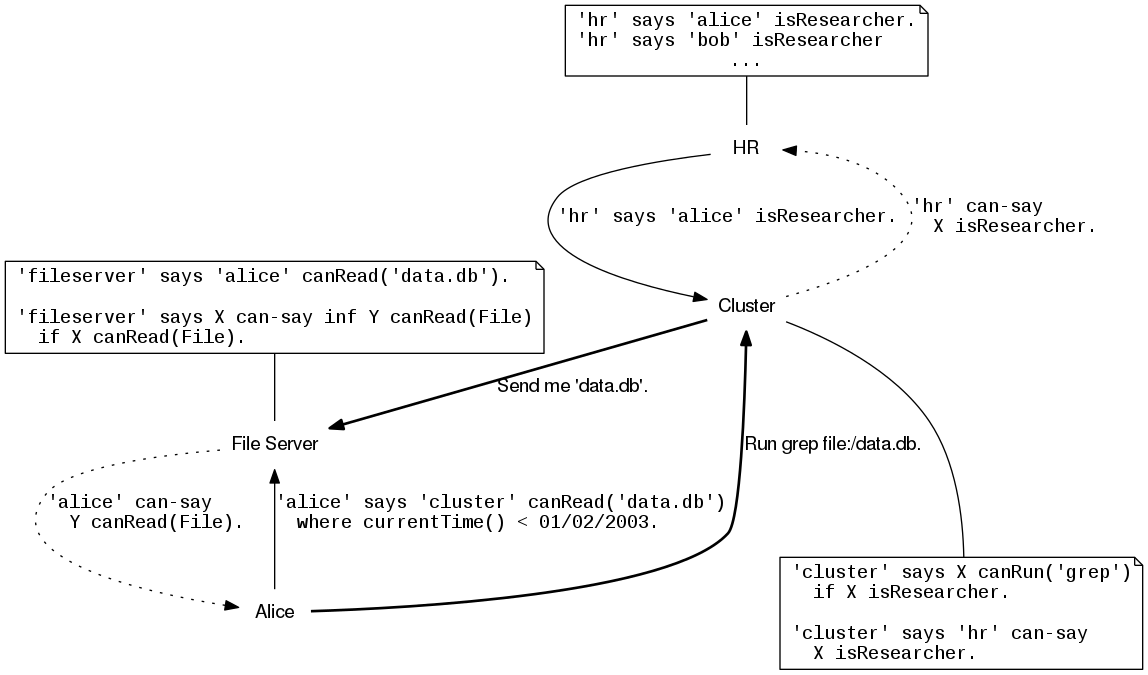
\includegraphics[width=\textwidth]{figures/secpal-example.png}
  \caption[Example of delegation on a cluster.]{Example of delegation when running a command on a cluster.  Bold links show requests, plain links show the sending of SecPAL statements, and dotted links indicate delegation relationships.  SecPAL assertions at each location are shown in notes.}
  \label{fig:delegation-example}
\end{figure}

Alice sends a request to the cluster to run a search on her data on the file-server.
The cluster has a SecPAL policy that only researchers can run the search:
\begin{lstlisting}
'cluster' says X canRun('grep')
  if X isResearcher.
\end{lstlisting}
and a rule that says only HR can say who is a researcher or not.
\begin{lstlisting}
'cluster says 'hr' can-say
  X isResearcher.
\end{lstlisting}
The cluster queries HR if Alice is a researcher or not and HR responds by sending the assertion that she is.
\begin{lstlisting}
'hr' says 'alice' isResearcher.
\end{lstlisting}
The cluster does not know how HR knows that Alice is a researcher, but
is content with HR's assertion that she is.  HR may have a SecPAL
instance and policy of their own to make this and send it to the
cluster, or they might be using a conventional database.  Provided
they give this signed SecPAL assertion to the cluster, it doesn't care
how they came by it.  The one limitation the cluster has is that it
\emph{must} be HR who tells them; HR cannot delegate the decision
further.

With the cluster convinced that Alice is authorized to run the search,
the cluster requests the database from the file server.  The file
server knows that Alice can read her data and that anyone who can read
a file is permitted to say who else can read it.
\begin{lstlisting}
'fileserver' says 'alice' canRead('data.db').
'fileserver' says X can-say inf Y canRead(File)
  if X canRead(File).
\end{lstlisting}
Using SecPAL, the file server, determines that Alice can say who can
read her data.  Alice provides the file server with a statement that
the cluster is authorized to read her file (for a short time
period).
\begin{lstlisting}
'alice says 'cluster' canRead('data.db')
  where currentTime() < 01/02/2003.
\end{lstlisting}
Dutifully the file server provides the cluster with the data
it required.  The cluster runs the search and hands the results back to Alice.

\begin{figure}
  \centering
  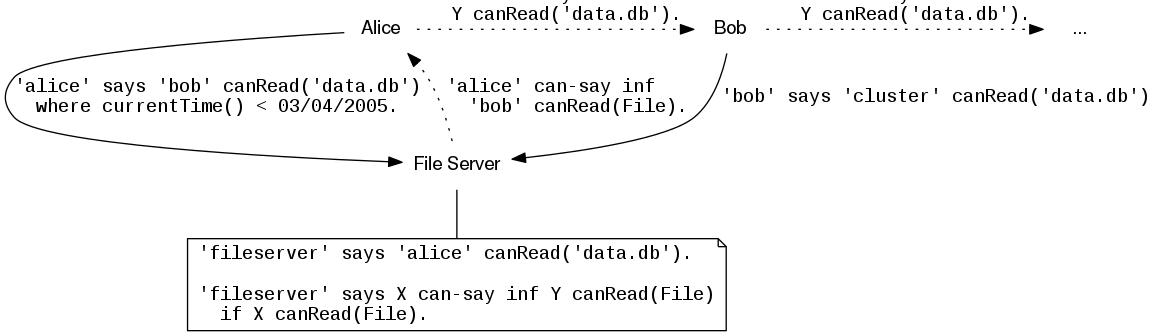
\includegraphics[width=\textwidth]{figures/secpal-example-delegation.png}
  \caption{Example of unbounded delegation.}
  \label{fig:unbounded-example}
\end{figure}

This simple example shows how different principals can make decisions using delegation mechanisms, and by sharing assertions.
SecPAL allows for more complicated delegation relationships, however. When checking who could access Alice's data, the file server allowed Alice the ability to delegate the decision of who could read her file by using the \texttt{can-say inf} verb.
Alice might allow Bob to share her data set with others who might also be allowed to share it for a limited time (\autoref{fig:unbounded-example}).

\begin{figure}
  \centering
  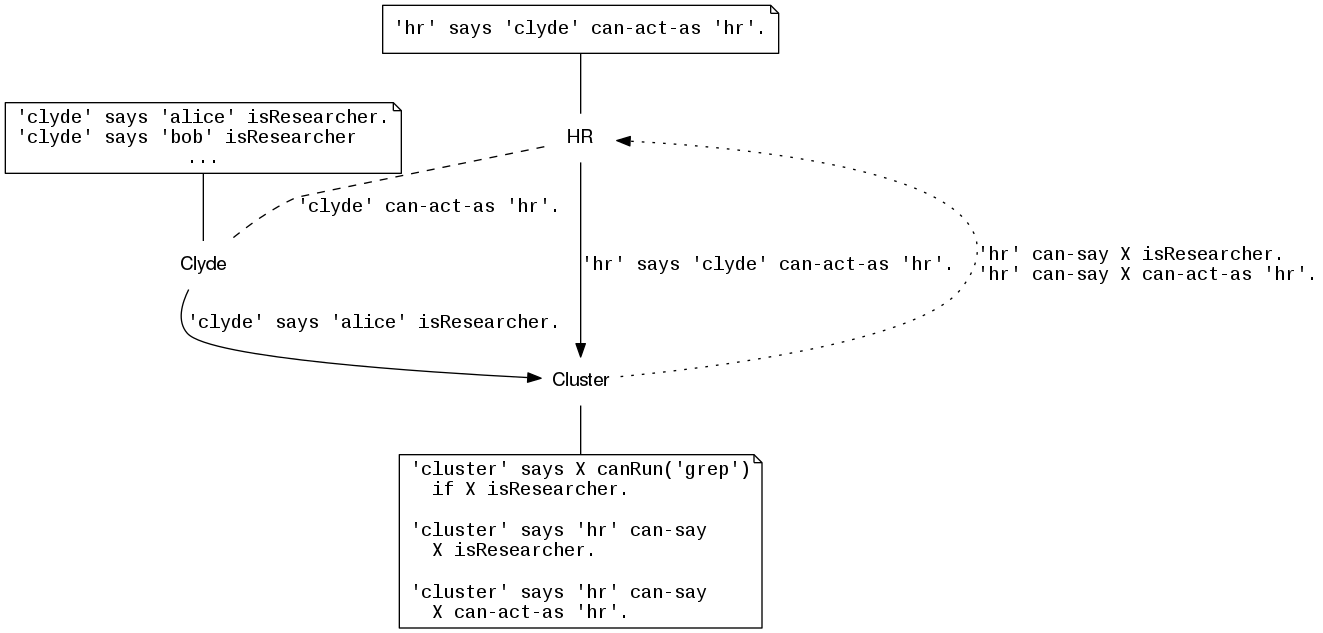
\includegraphics[width=\textwidth]{figures/secpal-example-roles.png}
  \caption[Example of delegation with roles.]{Example of delegation with roles.  Role relationships are shown with dashed links.}
  \label{fig:roles-example}
\end{figure}

An alternative to the delegation to the HR server to determine if
Alice was a researcher would be to use delegation with roles (shown in
\autoref{fig:roles-example}).  HR may consist of many principals.  The
cluster may be happy to accept the word of anyone who works in HR as
if they were HR.  To do this the cluster adds a delegation to HR that
they can name anyone who acts as them, and HR respond by saying that
Clyde can act for them.
\begin{lstlisting}
'cluster' says 'hr' can-say
  X can-act-as 'hr'.
'hr' says 'clyde' can-act-as 'hr'.
\end{lstlisting}
Now on the cluster Clyde's word is as good as HR's.
Clyde sends the necessary facts about Alice and the program can be run as before.
It is important to note that any restrictions on HR also apply to Clyde.  He still cannot delegate the decision further.

\begin{figure}
  \centering
  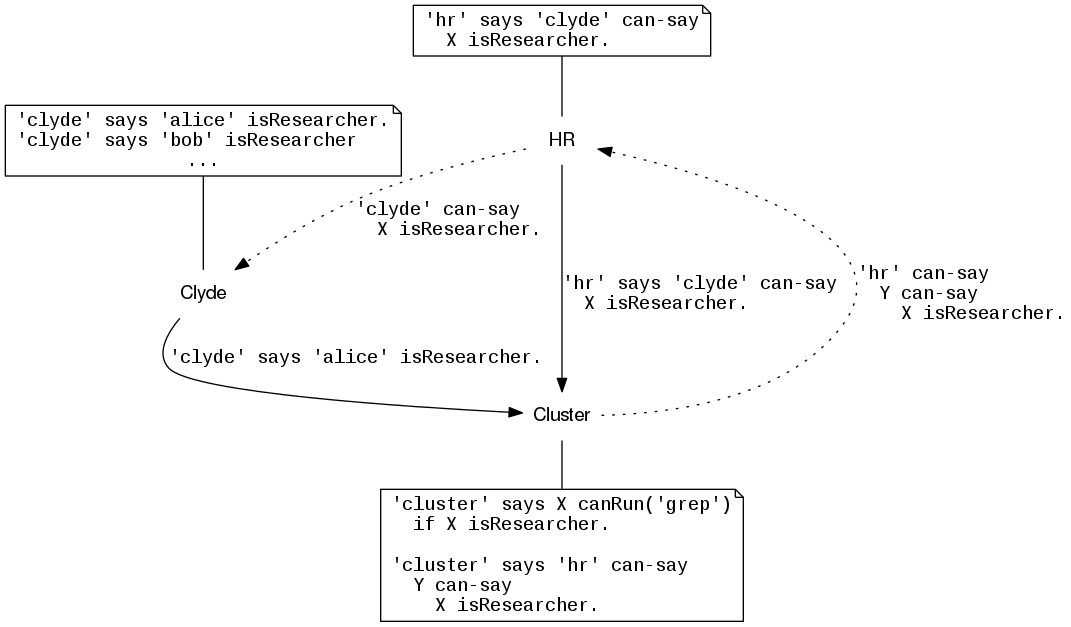
\includegraphics[width=\textwidth]{figures/secpal-example-delegation2.png}
  \caption{Example of depth bounded delegation.}
  \label{fig:depth-example}
\end{figure}

As an alternative to roles, depth-bounded delegation with the
\emph{can-say} statement could also have been used
(\autoref{fig:depth-example}).  In this case instead of delegating the
decision of who is a researcher to HR, the cluster delegates the
\emph{decision of who can make the decision} to HR.  HR makes the
delegation to Clyde, and the process continues as before.
Depth-bounded delegation allows delegation statements to be chained to
an arbitrary (but finite) depth, without allowing for unbounded
delegation.  It is often preferable to roles as it allows HR to
delegate some but not all decisions to others.  If the role assignment
is used then, on the cluster, anywhere \texttt{'hr'} follows the
\texttt{says} in an assertion, then it can be replaced with
\texttt{'clyde'}: making them effectively equivalent.

SecPAL's delegation mechanisms can describe a large number of
different relationships, whilst remaining conceptually and
semantically extremely simple.  This power makes SecPAL an exteremely
attractive authorization language for situations where entities are
distributed and there is no central decision maker: whatever
relationship each of the entities have SecPAL can describe it.

\section{Policy Languages}

\begin{figure}
  \centering\sffamily\scriptsize
  \begin{chronology}[5]{1987}{2017}{\textwidth}
    \event{1988}{X.509~}
    \event{1991}{A Calculus for Access Control~\cite{abadi_calculus_1991}}
    \event{1994}{Authentication in the Taos OS~\cite{wobber_authentication_1994}}
    \event{1996}{PolicyMaker~\cite{blaze_decentralized_1996}}
    \event{1998}{KeyNote~\cite{blaze_keynote:_1998}}
    \event{1999}{SPKI/SDSI}
    \event{2000}{Delegation Logic}
    \event{2001}{Ponder~\cite{damianou_ponder_2001}, XACML}
    \event{2002}{RT~\cite{li_design_2002}, Binder~\cite{detreville_binder_2002}}
    \event{2004}{Cassandra}
    \event{2005}{XACML 2.0}
    \event{2006}{SecPAL~\cite{becker_secpal:_2006}}
    \event{2008}{DKAL~\cite{gurevich_dkal:_2008}}
    \event{2009}{DKAL2~\cite{yuri_gurevich_dkal2---simplified_2009}, Ponder2~\cite{twidle_ponder2:_2009}, SecPAL4P~\cite{becker_framework_2009}}
    \event{2010}{XACML 3.0~\cite{oasis_extensible_2013}}
    \event{2011}{SecPAL4DSA~\cite{aziz_secpal4dsa:_2011}}
    \event{2013}{DKAL$\star$~\cite{jeannin_dkal*:_2013}}
    \event{2016}{AppPAL~\cite{hallett_apppal_2016}}
  \end{chronology}
  \caption{Timeline of the development of different policy languages.}
\end{figure}

This thesis focusses on an instantiation of SecPAL to describe the trust
relationships and decisions in the mobile ecosystem. In this section we provide
a survey of other policy languages and their geneology.

PolicyMaker~\cite{blaze_decentralized_1996} was created to give a language for
permitted actions. It grew out of the logics of authentication of Wobber, Abadi,
Burrows and Lampson~\cite{wobber_authentication_1994,abadi_calculus_1991}; as
well as a dissatisfaction with identification mechanisms. X.509 and PGP
certificates had given a mechanism for identifying users; at the time however,
they did not give any means to link the users to what users were allowed to do.

To describe the authorizations trust information is contained within assertions.
A collection of assertions form the policy. An assertion has a source (either
the local policy document or a public key). The source \emph{asserts} that a key
(or more complex arrangements such as three of four keys) is permitted to
perform any action that matches the \emph{filter}. The filter itself is
essentially an arbitrary program that can decide if an action is permitted.
Blaze~\etal~provide examples using regular expressions and a reduced version of
AWK~\cite{aho_awk-pattern_1979} they call \emph{AWKWARD}, though they note that
any programming language could be used. The collection of these authorizations
on a machine forms the policy for the device which can be queried by a
PolicyMaker key \emph{requesting} a given action.

Blaze~\etal~give an example of this scheme being used as part of an email
server. A user, Alice, identified by key \texttt{0x12345678} is permitted to
send emails with the from header set to Alice and the organisation set to Bob
Labs.

A PolicyMaker instance is installed on a server and allowed to receive queries and give answers.
The policy is installed on the server as follows:

\begin{lstlisting}
policy ASSERTS
  pgp:'0x12345678'
  WHERE PREDICATE=regexp:'(From: Alice) &&
    (Organization: Bob Labs)';
\end{lstlisting}

When Alice tries to send an email using a PolicyMaker enhanced SMTP
client she signs and sends her message using her key.  The mailserver
checks the signature and queries the policy server with her message:

\begin{lstlisting}
  pgp:'0x12345678'
  REQUESTS  'From: Alice
             Organization: Bob Labs

             Hello World!';
\end{lstlisting}

If Alice's request is accepted then the SMTP server will send the
message.  If it doesn't match the policy then it won't.

PolicyMaker was used as the basis for the KeyNote Trust Management
System~\cite{blaze_role_1999,blaze_keynote:_1998} which simplified the
filter languages from any arbitrary language to a purpose built one
based on C that always returned a boolean answer, allowed the policy
server to do the signature verification instead of the querying
application, and tweaked the syntax for readability.  It was designed
to trade some of the generality of PolicyMaker for a more realistic
scenario using public-key infrastructure.  The equivalent policy for KeyNote could be written:

\begin{lstlisting}
Authorizer: "POLICY"
Licensees: "RSA:abc123"

KeyNote-Version: "2"
Local-Constants: Alice="RSA:12345678" 
Authorizer: "RSA:abc123"
Conditions: (app_domain == "RFC822-EMAIL") &&
    (name="Alice") &&
    (organization="Bob Labs");
\end{lstlisting}

Checking whether a PolicyMaker or KeyNote policy is satisfied is
NP-hard~\cite{blaze_compliance_1998}.  It is not tractable as checking
PolicyMaker assertions can involve arbitrary programs written in
Turing complete languages.  Deciding whether a program will stop when
given an arbitrary input is analogous to the halting problem.  So in
general it is not known whether a PolicyMaker program which takes an
arbitrary request and an unconstrained set of checking functions will
terminate: it is undecidable.  Blaze~\etal{} give
some restrictions that guarantee polynomial time checking: a function
must be authentic (not fake another functions result), monotonic, and
run in polynomial time for all inputs pertinent to a request.  This
reduced the expressiveness however.

Another weakness of these languages is that they cannot express
general relationships as the subjects of the policy cannot be a
variable.  You cannot have, for example, a policy where the subject is
a set of users.  The example policy could not be written as
\emph{anyone working in R\&D can send email from Bob Labs.}  This
restriction made the languages less expressive than they might
otherwise have been.

%\subsection{SPKI/SDSI}

In contrast to PolicyMaker, SPKI/SDSI~\cite{ellison_spki_1999} was
designed to associate keys with roles.  A user, Alice with key~$K_A$,
can present a certificate that says she can act as a \emph{Bob Labs
employee} (authorized by Bob with key~$K_B$) for one~year.

\begin{equation*}
  (K_A,~\text{\tt BobLabsEmployee},~K_B,~1~\text{year})
\end{equation*}

Bob can also create authorization certificates to permit his employees
to send emails, and can optionally delegate the decision further.

\begin{equation*}
 (K_B,~(K_B,~\text{\tt BobLabsEmployee}),~\bot,~\text{\ttfamily send\_email},~1~\text{year})
\end{equation*}

Where PolicyMaker let an administrator check if a specific action was permitted
by a specific user, SPKI/SDSI let administrators associate users with roles and
roles with tasks. The SPKI/SDSI version of the email sending policy doesn't
specify that all emails sent by Employees must have a field listing the lab as
the sending organization; that part of the policy must be implemented by
whatever implemented the \texttt{send\_email} functionality. One of the large
advantages of SPKI/SDSI is that it allows a higher-level view of the policy by
associating groups of users with a role, and roles with allowed actions.

A weakness of SPKI/SDSI however was that the language was not designed
with formal semantics.  This meant that it was not possible to define
precisely what promises the language gave or how to extend it safely
or even exactly what it does.  All these things must be inferred from
RFC 2693 which loosely defined it~\cite{ellison_spki_1999}. There were
several later attempts to fit a semantics to the
language~\cite{joseph_y._halpern_logic_1999,abadi_sdsis_1998,howell_formal_2000},
however not all covered every aspect of SPKI/SDSIs features.

The focus on roles leads to the RT family of
languages~\cite{ninghui_li_design_2002}, which associates policy
decisions with roles similar to how \ac{RBAC} systems associate access
decisions to the roles a user holds.  Policies are expressed as Horn
clauses.  A rule such as:

\begin{lstlisting}[language=prolog]
Bob.employee :- alice.
Bob.employee.sendEmail :- Bob.employee.
\end{lstlisting}

Should be read as \emph{Bob says Alice is an employee.  Bob says an
employee can send emails if they are an employee.}  Li~\etal{}
describe many different variants of RT each with increasing numbers of
features.  The most basic variant is
\RT{0}{}~\cite{li_distributed_2003}, but \RT{1}{} adds support for
parameterized roles, and \RT{2}{} adds logical objects on top of the
roles.  As well as these variants, the RT family of languages have
support for optional feature sets: \RT{}{T} allows for policies with
thresholds (i.e. Alice can send an email if two out of three of the
board members approve it), \RT{}{C} adds constraints, and \RT{}{D}
adds delegation~\cite{ninghui_li_design_2002}.

Unlike PolicyMaker, the RT family of languages was tractable, they could guarantee
that a query will be answered soundly in polynomial time with respect to the
size of the policy. To give this guarantee trust languages some trust languages
such as Binder~\cite{detreville_binder_2002} and
Delegation~Logic~\cite{li_delegation_2003,li_practically_2000} had shown that
they could be reduced to Datalog, a database language with known complexity
guarantees and fast evaluation based on Prolog. One limitation of Datalog is
that it cannot describe structured data: for example consider an administrator
who wishes to write a policy rule that says Alice can send email between 9am and
5pm. We can imagine in the policy rule having some function to fetch the time
and another to compare whether it is within that range. In Datalog we cannot
trivially write this function and instead have to enumerate each possible time
in that domain and state whether it is within that period. More generally
whenever there is data that has structure such as file paths, times or numeric
intervals; Datalog databases can become large and start to become intractable.

To solve this problem Li~\etal{}~proposed a modified version of
Datalog called Datalog\textsuperscript{C}~\cite{li_datalog_2003},
based on Constraint
Datalog~\cite{revesz_constraint_1995,revesz_safe_1998}, that better
supported constraints and kept Datalog's tractability, with a focus on
the constraints typical to a policy languages instead of those for
database programming.

Datalog\textsuperscript{C} has also been used as a foundation for many
other policy languages including SecPAL based
languages~\cite{aziz_secpal4dsa:_2011,becker_secpal:_2006,becker_framework_2009}
and DKAL~\cite{gurevich_dkal:_2008}, as well as
Cassandra~\cite{becker_cassandra:_2004}.

Ponder, like SecPAL, was a language for specifying policies for distributed
systems~\cite{damianou_ponder_2001}. Ponder supports positive and negative
authorization, delegation, obligation, roles and constraints which are used to
extract the attributes of principals, as well as state and temporal information.
A policy that trainee engineers are not allowed to send emails could be written:

\begin{lstlisting}
inst auth- engineersCanEmail {
  subject e =/Engineer;
  target  /mail_server;
  action send_email();
  when e.status() == ``trainee'';
}
\end{lstlisting}

Since Ponder allowed positive and negative policies, conflicts could occur where
an entity satisfied rules that they both could and could not complete an action.
Ponder did not resolve the conflicts itself, but rather detected them using
static analysis and reports them to the policy author as bugs in the policy
specification. Ponder was followed by Ponder2~\cite{twidle_ponder2:_2009} which
simplified the language and enabled it to enforce policies in decentralized
environments. Ponder also provided a control language called \emph{PonderTalk}
that enabled the decision engine to send messages to the objects it was
managing.

Cassandra is a trust management language used to model large systems,
in particular the NHS Spine: a system designed to enable healthcare
workers to share patient
data~\cite{becker_cassandra:_2004,becker_cassandra:_2004-1}.  The
language is similar to the RT family, sharing both a backend and some
syntax, however Cassandra focuses on roles rather than general access
control mechanisms.  Rather than having principals hold or be given
roles, principals \emph{activate} roles when they need to act in that
capacity.  This allows a single principal to hold different roles with
different access capabilities at different times and at different
locations.  For example a \emph{hospital} \emph{admin} allows a
\emph{clinician} access to a \emph{patient}'s records if they
currently hold the role of \emph{Clinician} at the hospital, and can
\emph{activate} the role of \emph{Treating Clinician} for that patient
at this \emph{hospital}.

\begin{lstlisting}
hospital@admin.permits(clinician, Read-Records(patient)) <-
  hospital@hasActivated(clinician, Clinician(hospital)),
  hospital@canActivate(clinician, TreatingClinician(hospital, patient))
\end{lstlisting}

Cassandra allows for powerful control of different roles, and enables
delegation by allowing third-parties to activate and deactivate roles
on others.  It was applied successfully to modelling access control
with electronic healthcare records.

The DKAL family of
languages~\cite{jeannin_dkal*:_2013,gurevich_dkal:_2008,yuri_gurevich_dkal2---simplified_2009}
grew from SecPAL as a policy language for a distributed
system's interacting agents~\cite{blass_introduction_2012}. Assertions are
communicated as signed statements called \emph{infons} between principals. For
example Alice might wish to recommend Bob an app. Alice, therefore, sends to Bob
the infon:

\begin{lstlisting}
alice said com.rovio.angrybirds is a good app.
\end{lstlisting}

Bob is free to do with this information as he wishes.  He may be
willing to accept app recommendations from anyone and may have a rule
to learn that fact:

\begin{lstlisting}
with M: String, P: Principal
  upon
    P said M is a good app
  do
    learn P said M is a good app
\end{lstlisting}

DKAL2~\cite{yuri_gurevich_dkal2---simplified_2009} simplified the
language removing the constructs for roles that had been taken from
SecPAL but which they could not find a use for.  They also added
support for sending infons if the recipient has completed an action:
for example only sending an app recommendation if the recipient has
asked for it.
DKAL\textsuperscript{$\star$}~\cite{jeannin_dkal*:_2013} took these
ideas further and showed how DKAL programs that described how infons
should be shared could be used as executable protocols.

\end{document}

%%% Local Variables:
%%% mode: latex
%%% TeX-master: "../ch2"
%%% End:
